%%%%%%%%%%%%%%%%%%%%%%%%%%%%%%%%%%%%%%%%%
% Dreuw & Deselaer's Poster
% LaTeX Template
% Version 1.0 (11/04/13)
%
% Created by:
% Philippe Dreuw and Thomas Deselaers
% http://www-i6.informatik.rwth-aachen.de/~dreuw/latexbeamerposter.php
%
% This template has been downloaded from:
% http://www.LaTeXTemplates.com
%
% License:
% CC BY-NC-SA 3.0 (http://creativecommons.org/licenses/by-nc-sa/3.0/)
%
%%%%%%%%%%%%%%%%%%%%%%%%%%%%%%%%%%%%%%%%%

%----------------------------------------------------------------------------------------
%	PACKAGES AND OTHER DOCUMENT CONFIGURATIONS
%----------------------------------------------------------------------------------------

\documentclass[final,hyperref={pdfpagelabels=false}]{beamer}

\usepackage[orientation=portrait,size=a1,scale=1.3]{beamerposter} % Use the beamerposter package for laying out the poster with a portrait orientation and an a0 paper size

\usetheme{I6pd2} % Use the I6pd2 theme supplied with this template

\usepackage[english]{babel} % English language/hyphenation

\usepackage{amsmath,amsthm,amssymb,latexsym} % For including math equations, theorems, symbols, etc

%\usepackage{times}\usefonttheme{professionalfonts}  % Uncomment to use Times as the main font
%\usefonttheme[onlymath]{serif} % Uncomment to use a Serif font within math environments

\boldmath % Use bold for everything within the math environment

\usepackage{booktabs} % Top and bottom rules for tables

\graphicspath{{figures/}} % Location of the graphics files
\usepackage{graphicx}
\usepackage{wrapfig}

\usecaptiontemplate{\small\structure{\insertcaptionname~\insertcaptionnumber: }\insertcaption} % A fix for figure numbering

%----------------------------------------------------------------------------------------
%	TITLE SECTION 
%----------------------------------------------------------------------------------------

\title{\huge A Sphere Model for Atrial Fibrillation} % Poster title

\author{Tigany Zarrouk \& Mattia Gaggi } % Author(s)

\institute{Supervisor: Kim Christensen.  Condensed Matter Theory Group---Imperial College London} % Institution(s)

%----------------------------------------------------------------------------------------
%	FOOTER TEXT
%----------------------------------------------------------------------------------------

\newcommand{\leftfoot}{} % Left footer text

\newcommand{\rightfoot}{} % Right footer text


%----------------------------------------------------------------------------------------

\begin{document}

\addtobeamertemplate{block end}{}{\vspace*{2ex}} % White space under blocks

\begin{frame}[t] % The whole poster is enclosed in one beamer frame

\begin{columns}[t] % The whole poster consists of two major columns, each of which can be subdivided further with another \begin{columns} block - the [t] argument aligns each column's content to the top

\begin{column}{.02\textwidth}\end{column} % Empty spacer column

\begin{column}{.465\textwidth} % The first column

%----------------------------------------------------------------------------------------
%	OBJECTIVES
%----------------------------------------------------------------------------------------



%----------------------------------------------------------------------------------------
%	INTRODUCTION
%----------------------------------------------------------------------------------------
            
\begin{block}{Introduction}

\begin{itemize}
\item Atrial Fibrillation (AF) is a type of cardiac arrhythmia and one of the major causes of stroke and heart failure. AF is also the most widespread cardiac condition, with over 30 millions of people worldwide suffering from it. In the UK, expenses related to this disease account for more than $1\%$ of the total budget of the National Health Service, which is more than $800$ \textbf{ million pounds} .\\*
 Atrial fibrillation usually manifests itself in patients affected through alterations of the normal cardiac rhythm lasting short periods of time (also called fibrillation episodes).\\
\end{itemize}


\end{block}


\begin{block}{Phenomenology of the Heart}


	\begin{itemize}
	\item \textbf{\textit{Heart Beats Propagation}}: Each heart beat originates as an electric signal in the sinoatrial (SA) node that propagates first into the atria, then through the atrioventricular (AV) node, through Purkinje fibres 		and finally from the ventricular endocardium to the ventricular epicardium. The electric signal is conducted in the cardiac muscle cells thanks to the polarisation mechanism of the cell membrane. 

\begin{wrapfigure}{R}{0.3\textwidth}
\centering
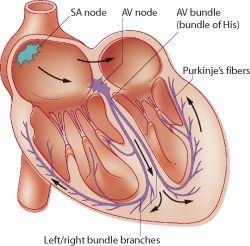
\includegraphics[width=0.25\textwidth]{heart}
\caption{\label{fig:frog1}This is a figure caption.}
\end{wrapfigure}


	\item \textbf{ \textit{Cells Excitation Rules}}: As the electric impulse propagates a single muscle cell goes through three stages:

		\begin{itemize}
 		 \item \textit{Excitable state}: the muscle cell is at rest with a negative built up potential.
  										
  		\item \textit{Excited state}: the muscle cell is excited by its excited neighbours and the Voltage of the cell is at its peak. 
  		\item \textit{Refractory state} :the muscle cell goes through a phase during which it can't be excited again - this period is called \textit{refractory period}. The \textit{refractory period} duration is related to the heart beat rate and this relationship is called \textit{restitution relationship}.
		\end{itemize}  





	\item \textbf{\textit{ How AF Occurs}}: AF is correlated to the amount of \textbf{ fibrosis} in the cardiac tissue which generates a process called \textit{ reentry}. \\
	During \textit{ reentry} the electric signal wavefront propagation breaks. 
	Even though many treatments have been developed, the mechanisms behind this condition are not completely understood and AF remains a major topic in medical research. \\
	%The current research revolves around three possible approaches:


%\begin{frame}
%\smartdiagram[bubble diagram]{Current research,
 %Physiological \\ models, Image-Based \\ Models, \textbf{ CA Models}, antiarrhythmic \\ drugs) }
% \end{frame}
 \item \textbf{\textit{Base for our Research}}: Our research is based on expanding on the work done by Kim Christensen which models the left atrium on a 2D surface.
	\end{itemize}

\end{block}
\begin{block}{Our Objectives}

\begin{enumerate}
\item Replicate the model of a 2D cardiac atrium from Christensen \emph{et al.}
\item  Translating the model onto a sphere in order to simulate the effects of a more realistic morphology. 
\item Incorporate restitution of heart cells into the original model (where the \textit{refractory period} is set to a constant).
\item Observe if there is a higher risk of Atrial fibrillation in the original model or in the new ones we developed.
\end{enumerate}


\end{block}


\begin{block}{Our Sphere model's Morphology}

%\centering
\begin{figure}
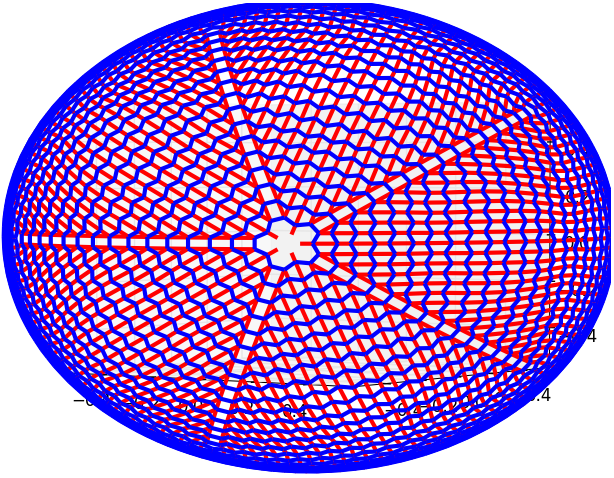
\includegraphics[width=0.7\linewidth]{connectome}
\caption{The structure of our sphere model on which we implemented electric impulse propagation using a network. The connections in red are differentiated from the connection in blue in order to introduce fibrosis in the model. Fibrosis is indeed modelled by removing a percentage of the red connections. }
\end{figure}

\end{block}


%\end{column}

%----------------------------------------------------------------------------------------

\end{column} % End of the first column

\begin{column}{.03\textwidth}\end{column} % Empty spacer column
 
\begin{column}{.465\textwidth} % The second column

%----------------------------------------------------------------------------------------
%	RESULTS
%----------------------------------------------------------------------------------------

%------------------------------------------------







\begin{block}{Model on a Sphere}




In research by Fedotov, a model of the atrium was constructed on the surface of a triangulated sphere to model spiral rotor waves on a closed, heterogeneous surface \cite{Fedotov}. Inspired by this research, we built a new model which translates Kim Christensen model of a two dimensional atrium on a sphere


%\end{block}
%------------------------------------------------
%\begin{block}{Results: Sphere and Previous model}

%\centering
\begin{figure}
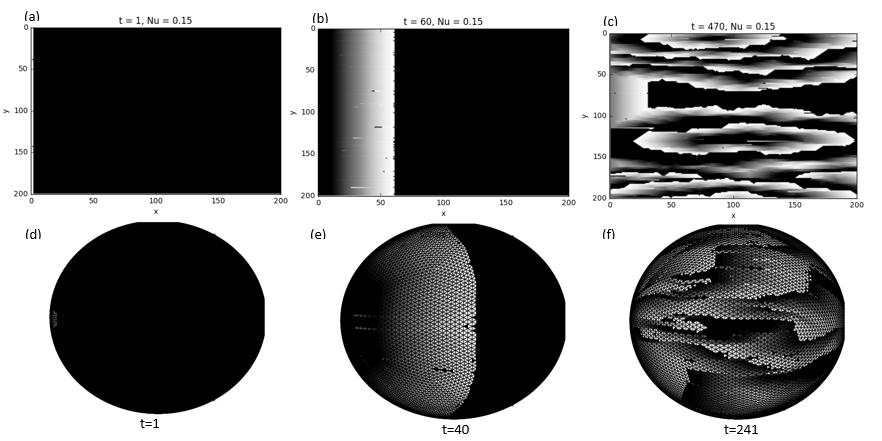
\includegraphics[width=0.8\linewidth]{combchristensenspherefib}
\caption{A comparison between Christensen \emph{et al.}'s model  (a, b and c)  and the sphere model (for d, e and f ) evolving in time in a not-healty atrium. Normal wavefront propagation is seen starting in the leftmost figures .In figures b,e the excitation wavefront propagates unevenly due to fibrosis, starting reentry. On the right AF has fully arisen from both models generating chaotic fibrillatory activity.}
\end{figure}

\end{block}

\begin{block}{Implementing Restitution }

In Christensen \emph{et al.}'s model, the refractory period of each muscle cell was always fixed, this is not what happens in a real heart.
In a real heart the refractory period depends on the heart beat rate and on the last time each cell it was excited. As already mentioned before he relationship between refractory period and heart beat rate is called restitution. We introduced restitution in In Christensen \emph{et al.}'s model in order to study its effects.
\end{block}


\begin{block}{Results: Risk of AF for the three models}

%\centering
\begin{figure}
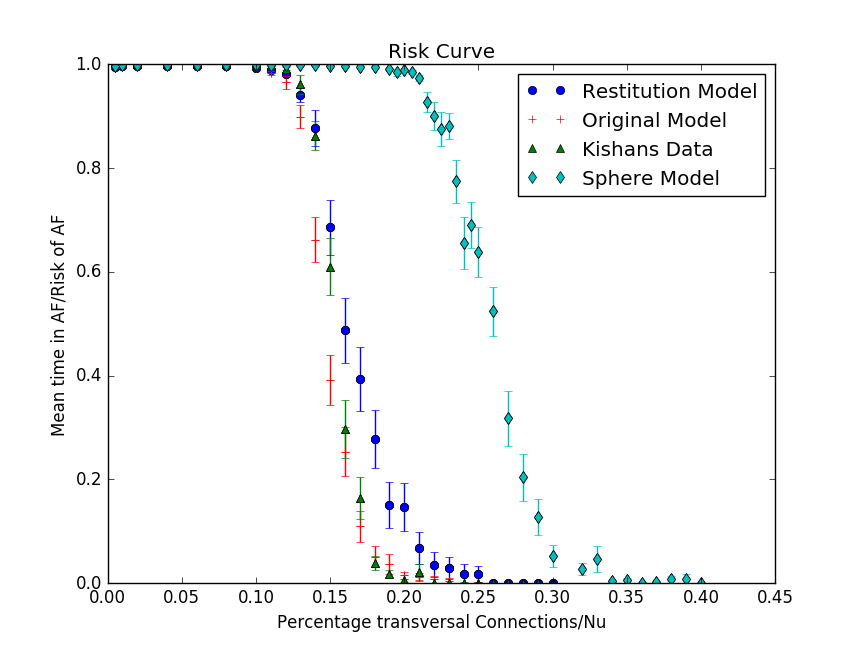
\includegraphics[width=0.65\linewidth]{xriskcurvesphere}
\caption{Risk of AF (defined as the fraction of time spent in fibrillation) for the three models studied (Prof Christensen's model, restitution curve model, sphere model) averaged over 100 simulations against percentage of transversal connections($\nu$) in the model. A healthy heart is expected to have $\nu$ close to 1 while a heart with fibrosis low $\nu$.}
\end{figure}

\end{block}

%----------------------------------------------------------------------------------------
%	CONCLUSION
%----------------------------------------------------------------------------------------

\begin{block}{Conclusion}

A simplified mechanism of AF had been achieved by Christensen \emph{et al.'s} model through the modelling of the atrium muscle tissue while incorporating the effects of fibrosis. We implemented this model by adding more realistic features by using a more realistic heart morphology and restitution. Our results show a higher risk of AF for the new models created.

\end{block}

%----------------------------------------------------------------------------------------
%	REFERENCES
%----------------------------------------------------------------------------------------

\begin{block}{References}
        
\nocite{*} % Insert publications even if they are not cited in the poster
\small{\bibliographystyle{unsrt}
\bibliography{sample1}}

\end{block}



%----------------------------------------------------------------------------------------
%	CONTACT INFORMATION
%----------------------------------------------------------------------------------------

%\setbeamercolor{block title}{fg=black,bg=orange!70} % Change the block title color

%\begin{block}{Contact Information}

%\begin{itemize}
%\item Web: \href{http://www.university.edu/smithlab}{http://www.university.edu/smithlab}
%\item Email: \href{mailto:john@smith.com}{john@smith.com}
%\item Phone: +1 (000) 111 1111
%\end{itemize}

%\end{block}

%----------------------------------------------------------------------------------------

\end{column} % End of the second column

\begin{column}{.015\textwidth}\end{column} % Empty spacer column

\end{columns} % End of all the columns in the poster

\end{frame} % End of the enclosing frame

\end{document}